\subsection{Wechselwirkung ionisierender Strahlung mit Materie}
In dem Versuch werden Übergänge in den beobachteten Stoffen über die Wechselwirkung emittierter $\gamma$-Quanten mit Materie nachgewiesen. Das Grundprinzip ist dabei, dass die Energie des Photons zunächst auf Elektronen übertragen wird und diese dann die Energie an das Detektormaterial abgeben. Im folgenden werden drei mögliche Wechselwirkungen skizziert.
\subsubsection{Compton-Effekt} 
Beim Compton-Effekt streut ein Photon an einem Teilchen (siehe Abbildung \ref{fig:compton}). Dabei wird ein gewisser Impuls vom Photon auf das Teilchen übertragen. Abhängig von Ablenkwinkel $\phi$ des gestreuten Photons lässt sich aus der (Vierer-)Impulserhaltung die Wellenlänge des gestreuten Photons zu
\begin{align}
  \lambda-\lambda_0=\frac{h}{mc}(1-\cos \phi)
  \label{eq:compton}
\end{align} 
berechnen. $h$ und $c$ sind dabei das Plancksche Wirkungsquantum und die Lichtgeschwindigkeit. $m$ ist die Masse des Teilchens. Der Ausdruck für die Wellenlängenverschiebung gilt in dem Bezugssystem, in dem das Teilchen zunächst ruht.
\begin{figure}[h]
  \centering
  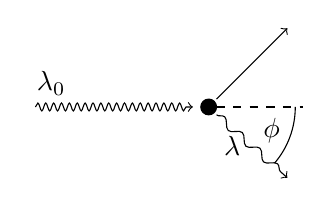
\begin{tikzpicture}[photon1/.style={decorate,decoration={snake, segment length=1mm, amplitude=0.5mm, post length=0.5mm}},photon2/.style={decorate,decoration={snake, segment length=3mm, amplitude=0.5mm, post length=0.5mm}}]
    \draw [->,photon1] (0,2)--(2,2);
    \draw [fill=black] (2.2,2) circle (0.1);
    \draw [->] (2.3,2.1)--(3.2,3);
    \draw [->,photon2] (2.3,1.9)--(3.2,1.1);
    \draw [dashed] (2.3,2)--(3.4,2);
    \draw (0.2,2.3) node {$\lambda_0$}; 
    \draw (2.5,1.5) node {$\lambda$};
    \draw (3.3,2) arc (0:-40.5:1.1);
    \draw (3,1.7) node {$\phi$};
  \end{tikzpicture}
  \caption{Compton-Effekt}
  \label{fig:compton}
\end{figure}

\subsubsection{Photoeffekt}
Beim Photoeffekt wird die Energie eines einfallenden Photons von einem Hüllenelektron eines Atoms absorbiert. Dadurch wird das Elektron ionisiert. Die kinetische Energie des Elektrons entspricht dann der ursprünglichen Energie des Photons abzüglich der Bindungsenergie des Elektrons.

\subsubsection{Paarbildung}
Bei der Paarbildung erzeugt ein energiereiches Photon ein Elektron-Positron-Paar. Die überschüssige Energie geht dabei in die kinetische Energie der erzeugten Teilchen. Ein Photon alleine kann noch nicht die Paarbildung auslösen. Es ist die Anwesenheit eines Atomkerns, eines Elektrons oder eines weiteren energiereichen Photons notwendig. Das Photon muss für die Paarbildung mindestens eine Energie haben, die der doppelten Ruhenergie des Elektrons entspricht (Energieerhaltung).

\subsection{Szintillationszähler}
Ein Szintillator weist ionisierende Teilchen nach. Die Teilchen regen die Atome im Szintillationsmaterial an. Nach einer mittleren Anregungsdauer fällt das Atom zurück in den Grundzustand und emittiert dabei ein Photon der entsprechenden Wellenlänge. Dieses Photon kann nun auch wieder weitere Atome anregen und es kommt zu einer Art Random-Walk. Um diesen zu unterbrechen, wird das Szintillationsmaterial schwach mit wellenlängenverschiebenden Molekülen dotiert. Trifft ein Photon auf ein solches, wird das Licht zu langwelligerem Licht umgewandelt. Dieses kann nicht vom Szintillator absorbiert werden und somit über einen Lichtleiter zu einer Photodiode gelangen. Diese erzeugt eine messbare elektrische Spannung. Der Prozess ist in Abbildung \ref{fig:szintillator} schematisch skizziert.
\begin{figure}[h]
  \centering
  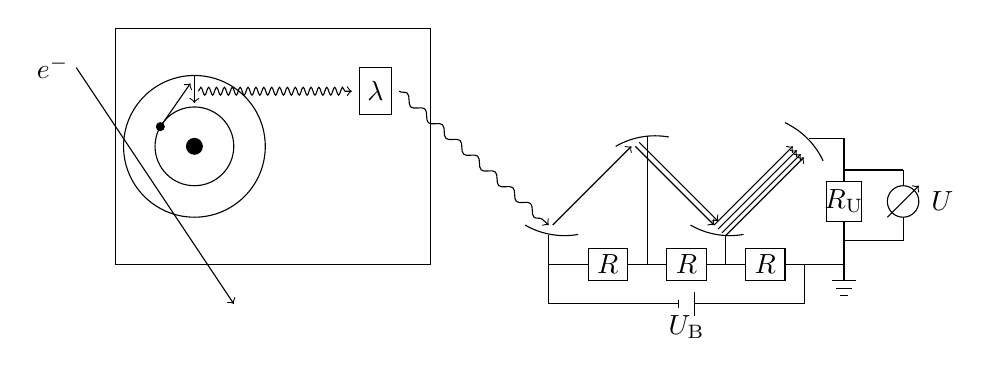
\begin{tikzpicture}[photon1/.style={decorate,decoration={snake, segment length=1mm, amplitude=0.5mm, post length=0.5mm}},photon2/.style={decorate,decoration={snake, segment length=3mm, amplitude=0.5mm, post length=0.5mm}}]
    \draw (0,0) rectangle (4,3);
    \draw [->] (-0.5,2.5)--(1.5,-0.5);
    \draw (-0.8,2.5) node {$e^-$};
    \draw (1,1.5) circle (0.9);
    \draw (1,1.5) circle (0.5);
    \draw [fill=black] (1,1.5) circle (0.1);
    \draw [fill=black] (1-0.5*1.732/2,1.5+1/4) circle (0.05);
    \draw [->] (1-0.5*1.732/2,1.5+1/4)--(0.95,2.3);
    \draw [->] (1,2.4) -- (1,2.05);
    \draw [->,photon1] (1.05,2.2) -- (3,2.2);
    \draw (3.1,1.9) rectangle (3.5,2.5);
    \draw (3.3,2.2) node {$\lambda$};
    \draw [->,photon2] (3.6,2.2)-- (5.5,0.5);
    \draw (5.2,0.5) arc (-120:-80:1);
    \draw [->] (5.55,0.5) -- (6.55,1.5);
    \draw (6.35,1.5) arc (120:80:1);
    \draw [->] (6.6,1.5) -- (7.6,0.5);
    \draw [->] (6.65,1.55) -- (7.65,0.55);
    \draw (7.3,0.5) arc (-120:-80:1);
    \draw [->] (7.65,0.45) -- (8.65,1.45);
    \draw [->] (7.6,0.5) -- (8.6,1.5);
    \draw [->] (7.7,0.4) -- (8.7,1.4);
    \draw [->] (7.74,0.36) -- (8.74,1.36);
    \draw (8.5,1.8) arc (65:25:1);
    \draw (9,0)--(8.5,0);
    \draw (8.75,0)--(8.75,-0.5)--(7.35,-0.5);
    \draw (7.15,-0.5)--(5.5,-0.5)--(5.5,0);
    \draw (8.5,0.2) rectangle (8,-0.2);
    \draw (8.25,0) node {$R$};
    \draw (8,0) -- (7.5,0);
    \draw (7.5,0.2) rectangle (7,-0.2);
    \draw (7.25,0) node {$R$};
    \draw (7,0) -- (6.5,0);
    \draw (7.75,0)--(7.75,0.375);
    \draw (6.75,0)--(6.75,1.635);
    \draw (6.5,0.2) rectangle (6,-0.2);
    \draw (6.25,0) node {$R$};
    \draw (6,0)--(5.5,0)--(5.5,0.375);
    \draw (7.35,-0.65)--(7.35,-0.35);
    \draw (7.15,-0.55)--(7.15,-0.45);
    \draw (7.25,-0.8) node {$U_\mathrm{B}$};
    \draw (9,0)--(9.25,0)--(9.25,0.55);
    \draw (9.03,0.55) rectangle (9.47,1.05);
    \draw (9.25,0.8) node {$R_\mathrm{U}$};
    \draw (9.25,1.05)--(9.25,1.6)--(8.8,1.6);
    \draw (9.25,0)--(9.25,-0.2);
    \draw (9.1,-0.2)--(9.4,-0.2);
    \draw (9.15,-0.3)--(9.35,-0.3);
    \draw (9.2,-0.4)--(9.3,-0.4);
    \draw (9.25,0.3)--(10,0.3);
    \draw (9.25,1.2)--(10,1.2);
    \draw (10,0.8) circle (0.2);
    \draw (10,0.3)--(10,0.6);
    \draw (10,1.2)--(10,1);
    \draw [->] (9.8,0.6)--(10.2,1);
    \draw (10.5,0.8) node {$U$};
  \end{tikzpicture}
  \caption{Beispiel für Signalerzeugung im Szintillator durch Elektron}
  \label{fig:szintillator}
\end{figure}

In diesem Versuch werden die Szintillationsdetektoren mit Hochspannung betrieben. Dadurch wird eine hohe Zeitauflösung bei Abgriff der Spannung an der Anode (Fast-Signal) erreicht. Durch die hohe Verstärkung des Signals im Photomultiplier ist die gemessene Spannung aber nicht mehr direkt proportional zu der ursprünglichen Photonenenergie und die Energieauflösung verschlechtert sich. Für Energiemessungen wird deshalb vor der Anode schon an einer der Dynoden die Spannung abgegriffen (Slow-Signal).

\subsection{Signalform}
Das Spektrum bei Einfall von monoenergetischen Photonen setzt sich aus einem kontinuierlichen und einem diskreten Teil zusammen. Der kontinuierliche Teil entsteht durch den Compton-Effekt. Nach Gleichung (\ref{eq:compton}) entsteht also ein kontinuierliches Spektrum bis zu der Maximalenergie bei Rückwärtsstreuung (an der so genannten Compton-Kante). Oberhalb dieser Energie entsteht eine (bis auf Verbreiterung durch Dopplerverschiebung) diskrete Linie durch die komplette Deposition der Photonenenergie in dem Detektor durch den Photoeffekt. Reicht die Photonenenergie für die Paarerzeugung aus entsteht zusätzlich ein Peak bei der Elektronenenergie. Dieser entsteht durch die auf die Paarerzeugung folgende Annihilation wodurch zwei Quanten mit einer Energie von jeweils etwa \SI{511}{\kilo\electronvolt} emittiert werden. Die Linie wird deshalb auch \SI{511}{\kilo\electronvolt}-Linie genannt. \\

Beim Einfall von Photonen verschiedener Energien überlagern sich die monoenergetischen Spektren.

\subsection{Einkanalanalysator und Koinzidenzmodul}
Für die Zählung der mit dem Detektor gemessenen Ereignisse werden die analogen Signale der Szintillatoren in digitale Signale umgewandelt. Dazu wird ein Einkanalanalysator (SCA) verwendet. Gibt der Szintillator ein Signal innerhalb eines einstellbaren Spannungsintervalls an den SCA, gibt dieser eine logische 1 in Form eines Rechteckpulses aus. Die Dauer dieses Rechteckpulses ist ebenfalls einstellbar.\\

Für die Lebensdauermessung ist man interessiert daran, ob zwei Ereignisse gleichzeitig (bzw. schnell hintereinander) passiert sind. Dazu werden Diskriminatoren genutzt, die einem logischen UND entsprechen.

\subsection{Vielkanalanalysator}
Für die Aufnahme von Energiepspektren wird ein Vielkanalanalysator (MCA) verwendet. Dieser hat zwei Eingänge, einen (logischen) Gate-Eingang und einen analogen Eingang. Liegt auf dem Gate-Eingang eine logische eins an wird der Zählstand des dem analogen Signal entsprechenden Kanal um eins erhöht. Zwischen Signalhöhe und dem entsprechenden Kanal besteht ein linearer Zusammenhang. 

\subsection{Zeit-Pulshöhen-Konverter}
Mit Hilfe des Zeit-Pulshöhen-Konverters (TAC) kann ein Zeitabstand zwischen zwei logischen Signalen in ein analoges Signal mit Signalstärke proportional zu dem Zeitabstand um. Die zwei logischen Eingänge des TAC entsprechen den Eingängen für das Start- und das Stop-Signal für die Zeitmessung. 

\subsection{Constant-Fraction-Diskriminator}
Für die Lebensdauermessung müssen die analogen Signale des Szintillationsdetektors mit einem Constant-Fraction-Diskriminator (CFD) in logische Signale für den TAC umgewandelt werden. Würde man dazu einen SCA wählen, wäre bei gleicher Signalform die Zeit der Auslösung abhängig von der Verstärkung des analogen Signals und der ursprünglichen Signalstärke. Um dies zu vermeiden gibt der CFD immer dann ein logisches Signal aus, wenn ein bestimmter Anteil $c$ (Constant Fraction) der Signalamplitude erreicht wird. Die Zeit der Auslösung ist somit nur Abhängig von der Signalform und unabhängig von der Skalierung des Signals. \\

In dem CFD wird das Eingangssignal ein zwei Teile gesplittet. Der eine Teil wird um eine Zeit, kleiner als die Anstiegszeit des Signals (die also schon vorher grob bekannt sein muss), verzögert. Der andere Teil des Signals wird mit $1/c$ skaliert und invertiert. Anschließend werden die beiden Signale addiert. Beim ersten Nulldurchgang des resultierenden Signals wird das logische Signal ausgegeben.

\subsection{Zerfallsschemata von $^{133}$Ba und $^{22}$Na}
\begin{figure}[h]
  \centering
  \begin{subfigure}[h]{0.5\textwidth}
    \centering
    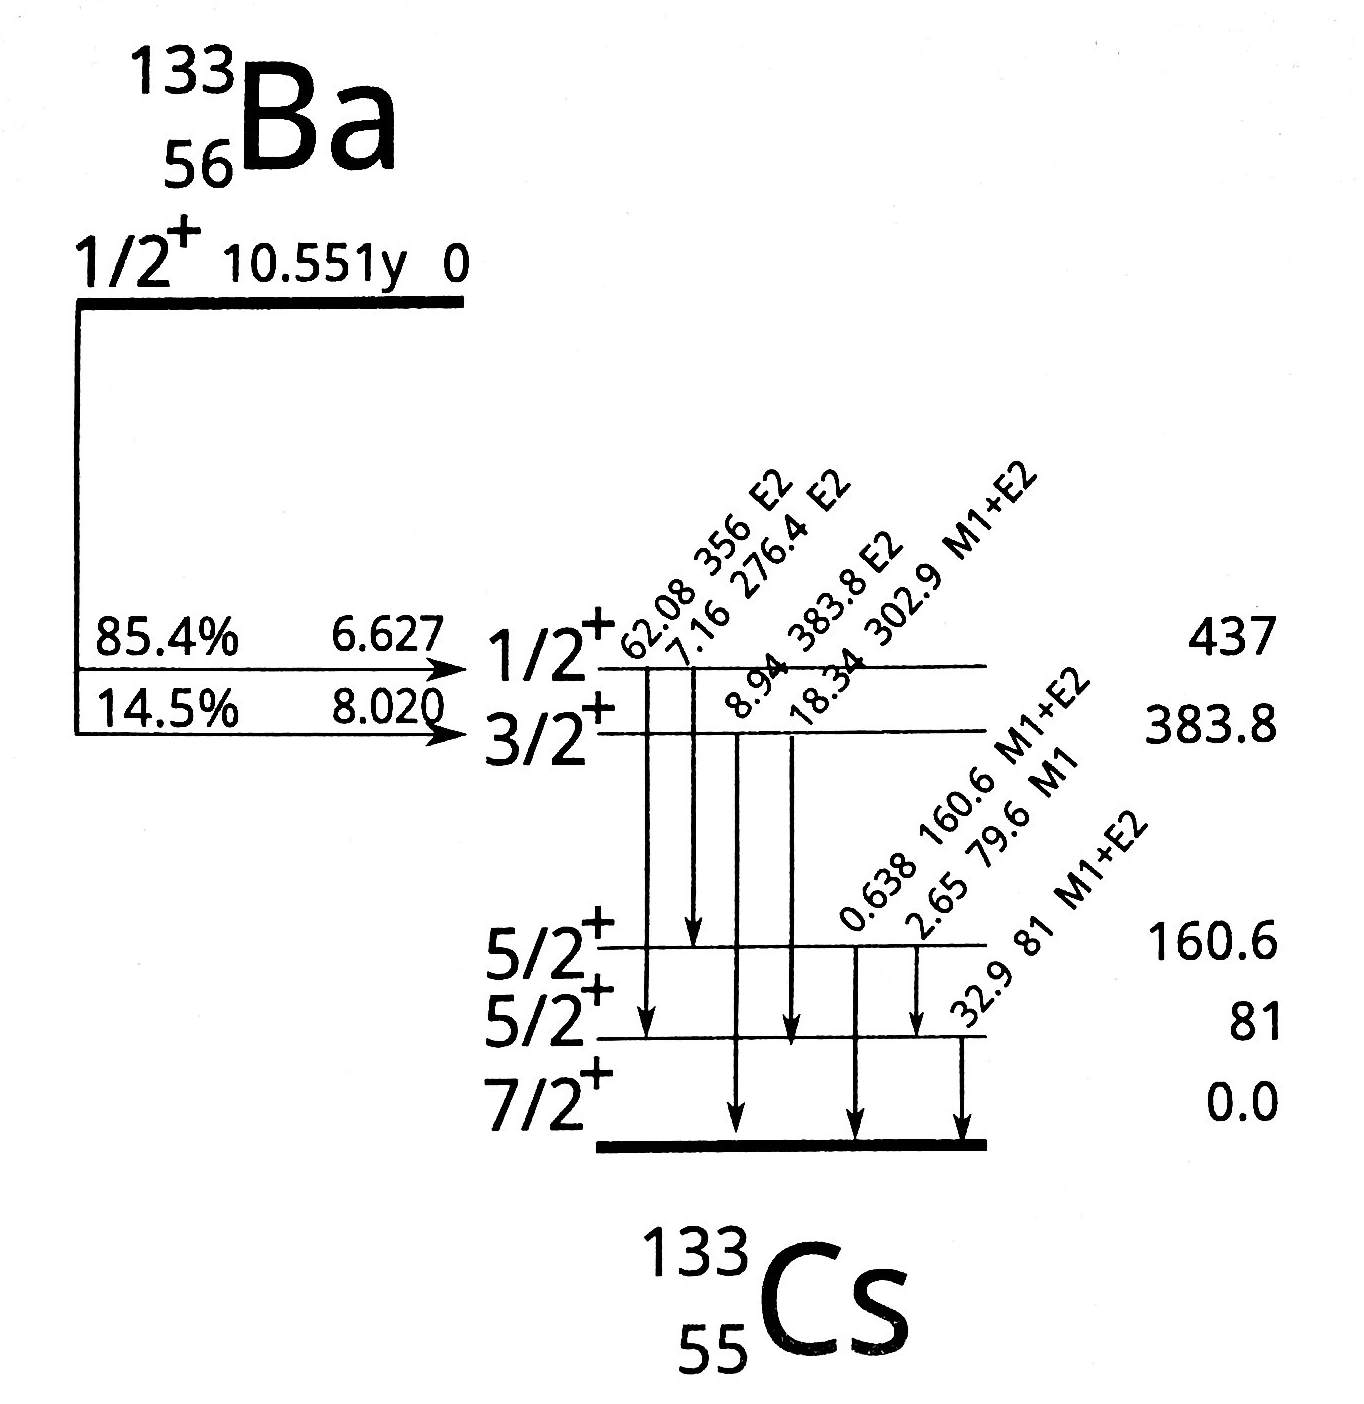
\includegraphics[width=0.9\textwidth]{data/ba_scheme.png}
  \end{subfigure}%
  \begin{subfigure}[h]{0.5\textwidth}
    \centering
    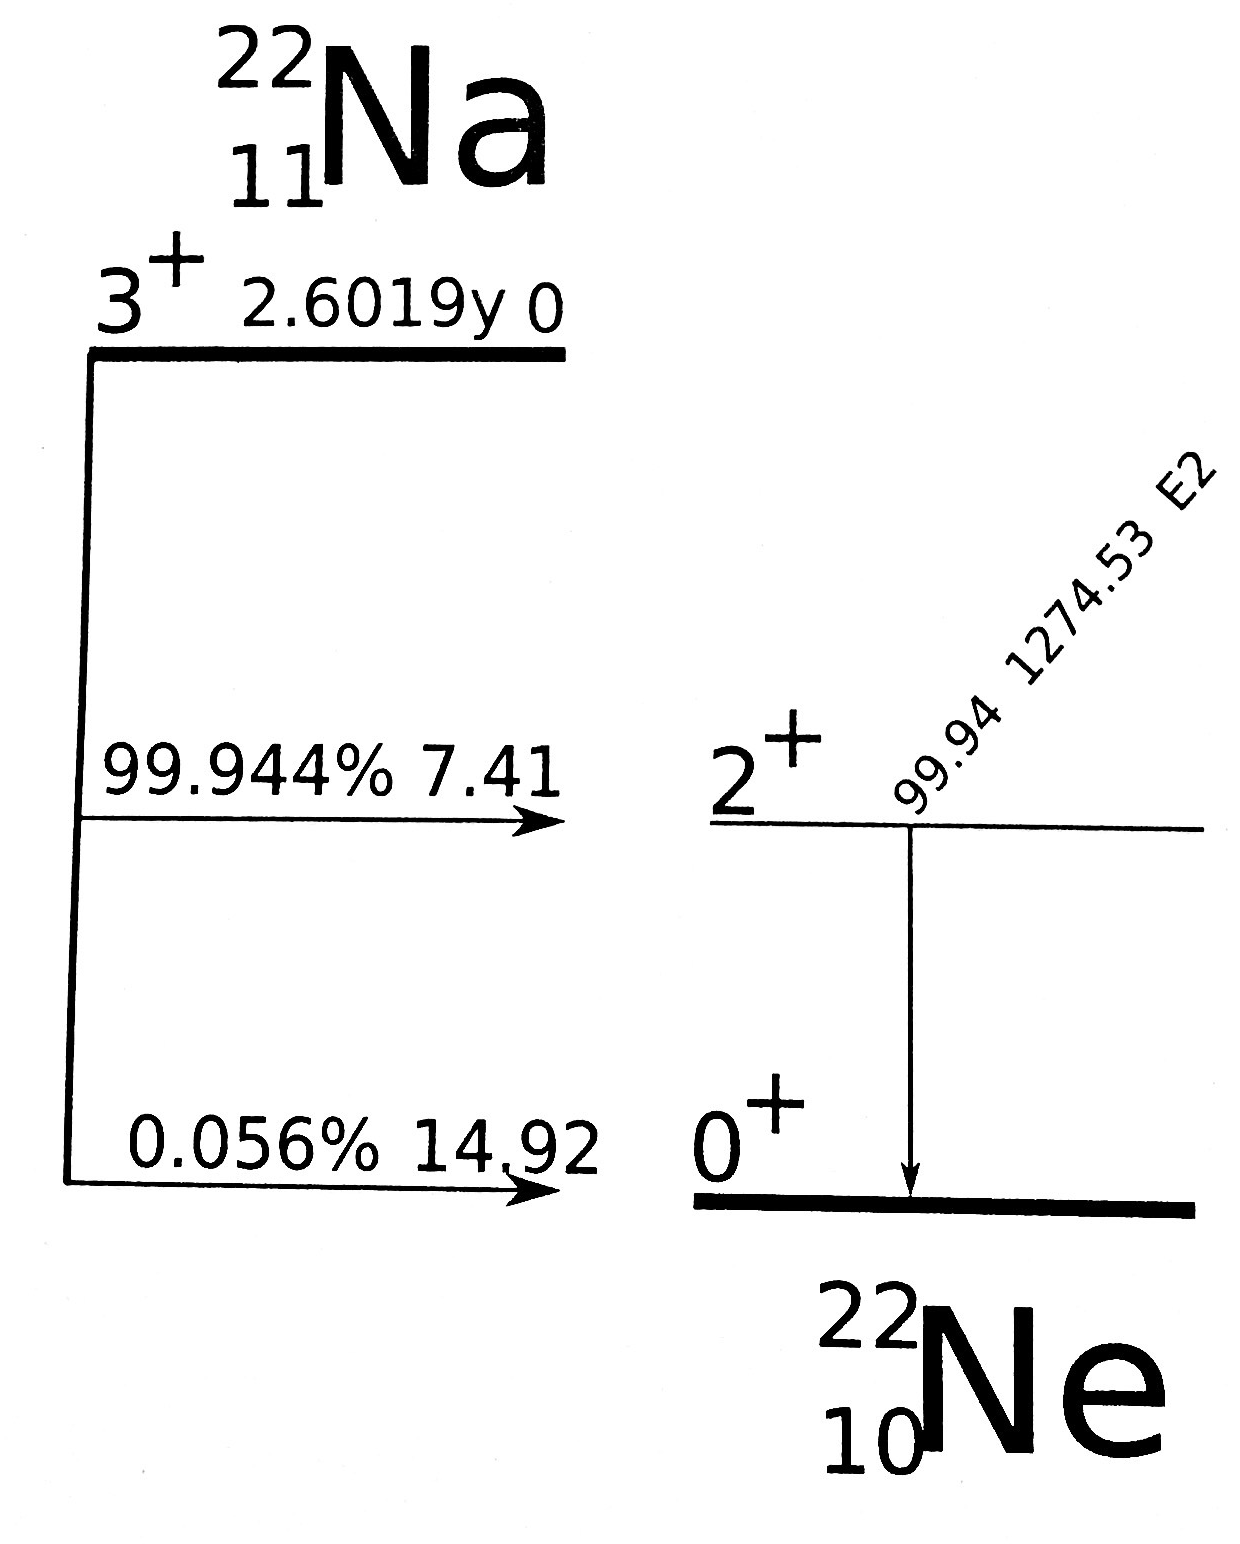
\includegraphics[width=0.7\textwidth]{data/na_scheme.png}
  \end{subfigure}
  \caption{Zerfallschemata von $^{133}$Ba und $11{22}$Na aus \cite{praktikumsheft}}
  \label{fig:scheme}
\end{figure}   
Das Zerfallschema von $^{133}$Ba ist in Abbildung \ref{fig:scheme} zu sehen. Über Elektroneneinfang zerfällt es zunächst in einen angeregten Zustand von $^{133}$Ba. Dieser kann dann durch $\gamma$-Übergänge über verschiedenen niedrigere Zustände bis zum Grundzustand zerfallen. Die Übergangsenergien reichen dabei nicht für die Paarproduktion aus. Es wird also keine \SI{511}{\kilo\electronvolt}-Linie im Spektrum erwartet. \\

In dem Versuch wird die Lebensdauer des ersten angeregten Zustandes mit einer Energie von \SI{81}{\kilo\electronvolt} über dem Grundzustand gemessen. Das Startsignal für die Zeitmessung gibt dabei das $\gamma_8$-Photon, welches die Bevölkerung des relevanten Zustandes signalisiert. Das Stopsignal gibt dann ein $\gamma_3$-Photon, welches die Entvölkerung signalisiert. \\

$^{22}$Na zerfällt über Elektroneneinfang zu dem Grundzustand oder dem angeregten Zustand von $^{22}$Ne. Über einen hochenergetischen $\gamma$-Zerfall kann der angeregte Zustand in den Grundzustand zerfallen. Die Energie des $\gamma$-Quants reicht dabei für die Paarproduktion aus und der \SI{511}{\kilo\electronvolt}-Peak wird im Spektrum erwartet.
